\documentclass{article}
\usepackage[english]{babel}
\usepackage{geometry}
\usepackage{amssymb}
\usepackage{xcolor}
\usepackage{booktabs}
\usepackage{graphicx}
\usepackage{float}
\usepackage{caption}
\usepackage{svg}

\usepackage{hyperref}
\captionsetup[figure]{hypcap=false}  % disabilita hypcap per figure
\captionsetup[table]{hypcap=false}

\setcounter{page}{0}

% \geometry{
%	left=.7in,  
%	right=.7in, 
%	top=.7in,   
%	bottom=.7in,
% }


\title{Quantum Effects in Materials: From Theory to Modelling Part B: LAB report}
\author{Alessio Cimma}

\begin{document}

\maketitle

\tableofcontents
\newpage

\section{Functionals (theory)}

Since there are many ways to calculate the informations of molecules and crystals, many functionals exist.
The way they work are different, based on different approaches for reaching the same goals.
The main difference lies in how the Hamiltonian is approximated. 
 
The functionals used during this project where the following, with a brief explanation of each method:
\begin{itemize}
	\item Hartree - Fock (HF): Basic functional, calculates very well the exchange energy but the correlation energy is not considered. Computationally expensive.
	\item PBE: More advanced approach, uses the Gradient Generalized Approximation (GGA). It's extremely fast, but tends to over-delocalize electronic densities, leading to inaccuracies in exchange-correlation interactions.
	\item PBE0 - D3: Hybrid functional between PBE and HF (25\%), takes the best of both worlds, considering correctly correlation-exchange energies. Since it has an HF part, it is computationally expensive.
	\item SVWN: Advanced approach. Considers both exchange and correlation energies. In this work it has been tested against the others to evaluate its performance. 
\end{itemize}

\begin{figure}[ht]
	\centering
	\includegraphics[width=0.5\textwidth]{../images/crystal.png} 
	\caption{Crystalline structure of $CeO_2$ (100), obtained from CRYSPLOT}
	\label{fig:crystal_ce02}
\end{figure}

\newpage
\section{Objectives \& Computational Set-up}
\subsection{Objectives}
In this work will be reported different properties of the crystalline structure $CeO_2$ computed using different functionals. A brief explanation on the results will follow.
Here's the list of properties:
\begin{itemize}
	\item Worth of Geometry Optimization 
	\item Single Point calculation
	\item Band structure 
	\item Density of States
	\item Charge Density
	\item Vibrational spectra
	\item Performances 
\end{itemize}

\subsection{Basis set choice}

The choice of using a single basis set instead of investigating different effects given by variable basis sets was given by the complexity of this system, about which the availability of basis sets was not so wide.

Because of the high number of functions needed to describe heavy atoms like Cerium, a pseudo-potential technique was used in order to define the basis set exploited in this report, where the core states are described in a less computational costly way.

\vspace{15pt}

\noindent The basis set used is the following:
\begin{itemize}
	\item Ce\_pob\_TZVP\_rev2 (Cerium)
	\item O\_pob\_TZVP\_rev2 (Oxygen)
\end{itemize}

\subsection{Geometry Optimization}

Inserting the keyword \texttt{OPTGEOM} after the geometry block in the input file, the total energy was minimized reaching the most stable configuration, as seen in Table \ref{tab:total_E}.

\begin{table}[H]
	\centering
	\begin{tabular}{llrrrr}
		\toprule
		& PBE0-D3 & PBE & SVWN & HF \\
		\midrule
		Total E (Ha) & -625.6031 & -625.6279 & -624.2352 & -623.5622 \\
	\end{tabular}	
	\caption{Results of Total Energy calculations across different functionals}
	\label{tab:total_E}
\end{table}

\noindent Different functionals had different results as reported in Table \ref{tab:geom_opt} and visually in the following sections:

\begin{table}[H]
    \centering
    \begin{tabular}{ccccc}
\toprule
N° CYCLES & HF & PBE & PBE0-D3 & SVWN \\
\midrule
0 & -625.60061106284 & -625.62786242137 & -624.23246794512 & -623.56221081248 \\
1 & -625.60301777511 & -625.62786231396 & -624.23517964377 & -623.56221060938 \\
2 & -625.60320214065 & -625.62786240368 & -624.23551479331 & -623.56221093063 \\
3 & -625.60320342391 & -625.62785897518 & -624.23551456006 & -623.56221094929 \\
4 & -625.60305428822 &   & -624.23551498470 & -623.56223235987 \\
5 & -625.60305448049 &   & -624.23551500618 & -623.56223109411 \\
6 & -625.60305151909 &   & -624.23551498133 & -623.56223120941 \\
7 &   &   & -624.23551497702 & -623.56223102610 \\
8 &   &   & -624.23519882041 & -623.56223133812 \\
9 &   &   & -624.23519908332 & -623.56223126704 \\
10 &   &   & -624.23519903774 &   \\
11 &   &   & -624.23519938698 &   \\
\bottomrule
\end{tabular}

    \caption{Geometry Optimization steps.}
    \label{tab:geom_opt}
\end{table}

\subsubsection{HF}
\begin{minipage}[t]{0.55\textwidth}
	\vspace{-\topskip}
	\includegraphics[width=1\textwidth]{../images/HF.png}
	\captionof{figure}{Geom. Opt. using HF}
	\label{fig:opt_HF}
\end{minipage}
\hfill
\begin{minipage}[t]{0.4\textwidth}
	\vspace{-\topskip}
	\vspace{20pt}
	There was no noticeable improving until the 4th cycle, after which a convergence was found.
\end{minipage}

\subsubsection{PBE}
\noindent\begin{minipage}[t]{0.55\textwidth}
	\vspace{-\topskip}
	\includegraphics[width=1\textwidth]{../images/PBE.png}
	\captionof{figure}{Geom. Opt. using PBE}
	\label{fig:opt_PBE}
\end{minipage}
\hfill
\begin{minipage}[t]{0.4\textwidth}
	\vspace{-\topskip}
	\vspace{20pt}
	Unfortunately the PBE functional had a strange spike at 3rd cycle, exiting the convergence stage. 
\end{minipage}

\subsubsection{PBE0-D3}
\noindent\begin{minipage}[t]{0.55\textwidth}
	\vspace{-\topskip}
	\includegraphics[width=1\textwidth]{../images/PBE0.png}
	\captionof{figure}{Geom. Opt. using PBE0 - D3}
	\label{fig:opt_PBE0}
\end{minipage}
\hfill
\begin{minipage}[t]{0.4\textwidth}
	\vspace{-\topskip}
	\vspace{20pt}
	The PBE0-D3 functional worked fine, following the classical convergence path.
\end{minipage}

\subsubsection{SVWN}
\noindent\begin{minipage}[t]{0.55\textwidth}
	\vspace{-\topskip}
	\includegraphics[width=1\textwidth]{../images/SVWN.png}
	\captionof{figure}{Geom. Opt. using SVWN}
	\label{fig:opt_SVWN}
\end{minipage}
\hfill
\begin{minipage}[t]{0.4\textwidth}
	\vspace{-\topskip}
	\vspace{20pt}
	The SVWN functional had the longest convergence, but reaching a good result nonetheless.
\end{minipage}

\subsubsection{Comparison}

The optimization by itself in most cases leads to the minimum of the final energy. 
However, by comparing each functional with eachother, it's possible to observe a much bigger difference in energies between the functional chosen rather than in the optimization obtained. 

%FRANCESCA: this implies that the optimization path is neglected with respect to the final energy of each functional. This is way ...

In this specific case, the comparison leads to believe that the Geometry Optimization does not influence the outcome in a significant way, suggesting that it may be omitted without loss of information, since the chosen functional has a much bigger impact on the final result.

\vspace{15pt}

\noindent Additionally, the calculations performed without Geometry Optimization were generally three times faster. However, the results are not reported, as in this report the focus was solely on analyzing the optimized results.


\begin{figure}[ht]
	\centering
	\includegraphics[width=0.9\textwidth]{../images/Comparison.png}
	\caption{Comparison of functionals and their optimizations}
	\label{fig:func_comparison}
\end{figure}

\newpage
\section{Single Point calculation}
The following properties were selected to be reported:
\begin{itemize}
	\item Total Energy (reported in the previous section)
	\item Orbitals Overlap
	\item Mulliken population
	\item Band Gap
	\item Performances (TCPU)
\end{itemize}

\subsection{Overlap}

The trend in orbital overlap—largest in HF, smallest in PBE, with PBE0-D3 and SVWN in between—reflects how each method treats exchange and correlation. HF's exact exchange localizes orbitals, increasing overlap, while PBE's semi-local approach leads to over-delocalization and reduced overlap. PBE0-D3 and SVWN balance these effects, yielding intermediate values.

\begin{table}[H]
	\centering
	\begin{tabular}{llrrrr}
		\toprule
		 & PBE0-D3 & PBE & SVWN & HF \\
		\midrule
		OVPOP Ce-O & 0.010 & 0.024 & 0.008 & -0.006 \\
	\end{tabular}	
	\caption{Results of Overlap calculations (Ce-O) across different functionals}
	\label{tab:overlap_Ce_O}
\end{table}
\begin{table}[H]
	\centering
	\begin{tabular}{llrrrr}
		\toprule
		 & PBE0-D3 & PBE & SVWN & HF \\
		\midrule
		OVPOP O-O & -0.032 & -0.021 & -0.029 & -0.037 \\
	\end{tabular}	
	\caption{Results of Overlap calculations (O-O) across different functionals}
	\label{tab:overlap_O_O}
\end{table}

\subsection{Mulliken population}

The Mulliken population analysis returns the net charge of each atom. The results are consistent across different functionals. Notice that the net charge of the $Ce$ is halfed respect to it's atomic number, this is due to stoichiometric reasons.

\begin{table}[H]
	\centering
	\begin{tabular}{llrrrr}
		\toprule
		 & PBE0-D3 & PBE & SVWN & HF \\
		\midrule
		Mulliken charges(Ce) & 27.755 & 27.992 & 28.043 & 27.252 \\
	\end{tabular}	
	\caption{Results of Overlap calculations (Ce-O) across different functionals}
	\label{tab:mulliken_Ce}
\end{table}
\begin{table}[H]
	\centering
	\begin{tabular}{llrrrr}
		\toprule
		& PBE0-D3 & PBE & SVWN & HF \\
		\midrule
		Mulliken charges(O) & 9.123 & 9.004 & 8.979 & 9.374 \\
	\end{tabular}	
	\caption{Results of Overlap calculations (O-O) across different functionals}
	\label{tab:mulliken_O}
\end{table}

\subsection{Band Gap}

The band gap has been an interesting property to analyze, since very big differences came out.
From literature the reference value of band gap for bulk $CeO_2$ is around 3.9 eV \cite{ceo2_band_gap}.
As expected, the HF functional highly overestimates the band gap due to the lack of the correlation term. On the other hand, PBE and SVWN underestimate the energy. The best result is obtained with PBE0-D3. 

\begin{table}[H]
	\centering
	\begin{tabular}{llrrrr}
		\toprule
		 & PBE0-D3 & PBE & SVWN & HF \\
		\midrule
		BAND GAP(eV) & 4.0991 & 1.8830 & 2.0214 & 14.1186 \\
	\end{tabular}	
	\caption{Results of Band Gap calculations across different functionals}
	\label{tab:band_gap}
\end{table}

\subsection{Performances (TCPU)}

As mentioned before, the HF functional has the biggest computational requirements, followed by the PBE0-D3, which again, is partly made from HF calculations. SVWN is an advanced method, hence it's explained why it's not the fastest functional. The PBE is the cheapest functional. It turns out that in general the best results are obtained with PBE0-D3, while the best cost-performance ratio is obtained with SVWN functional.

\begin{table}[H]
	\centering
	\begin{tabular}{llrrrr}
		\toprule
		 & PBE0-D3 & PBE & SVWN & HF \\
		\midrule
		TCPU [s] & 1864.71 & 334.54 & 770.92 & 2857.84 \\
	\end{tabular}	
	\caption{Time needed for calculations across different functionals}
	\label{tab:TCPU}
\end{table}

\newpage
\section{Band Structure}

From the following plots it is noticeable that the \textbf{HF} functional (Fig.\ref{fig:bands_HF}) places the conduction bands extremely above the Fermi Energy, confirming the expected overestimated band gap. The other functionals as well did not approach the theoretical result ($\sim$3.9 eV). The best band gap evaluation has been performed by \textbf{PBE0-D3} (Fig.\ref{fig:bands_PBE0D3}), with a difference of $\sim$0.2 eV from the reference value.

\vspace{15pt}

\noindent\begin{minipage}{0.45\textwidth}
	\centering
	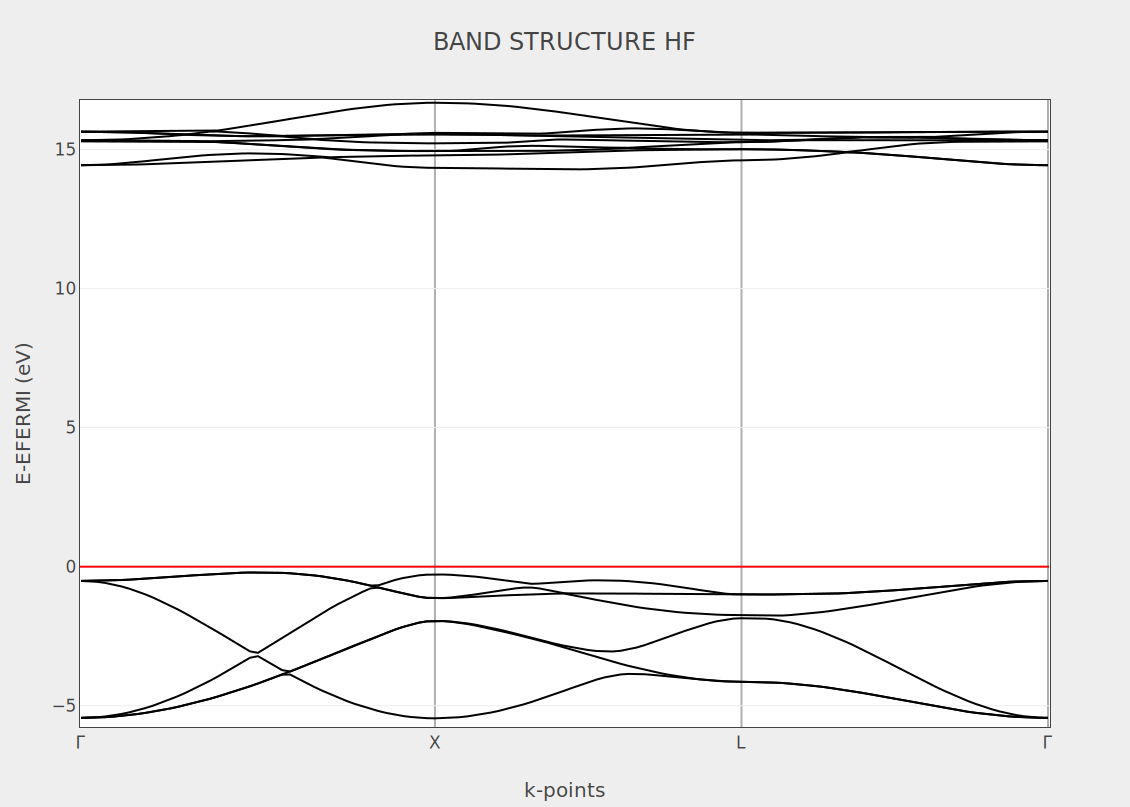
\includegraphics[width=1\textwidth]{../images/BANDS/BAND_STRUCTURE_HF.jpeg}
	\captionof{figure}{Reported Band Structure of $CeO_2$ using HF}
    \label{fig:bands_HF}
\end{minipage}
\hfill
\begin{minipage}{0.45\textwidth}
	\centering
	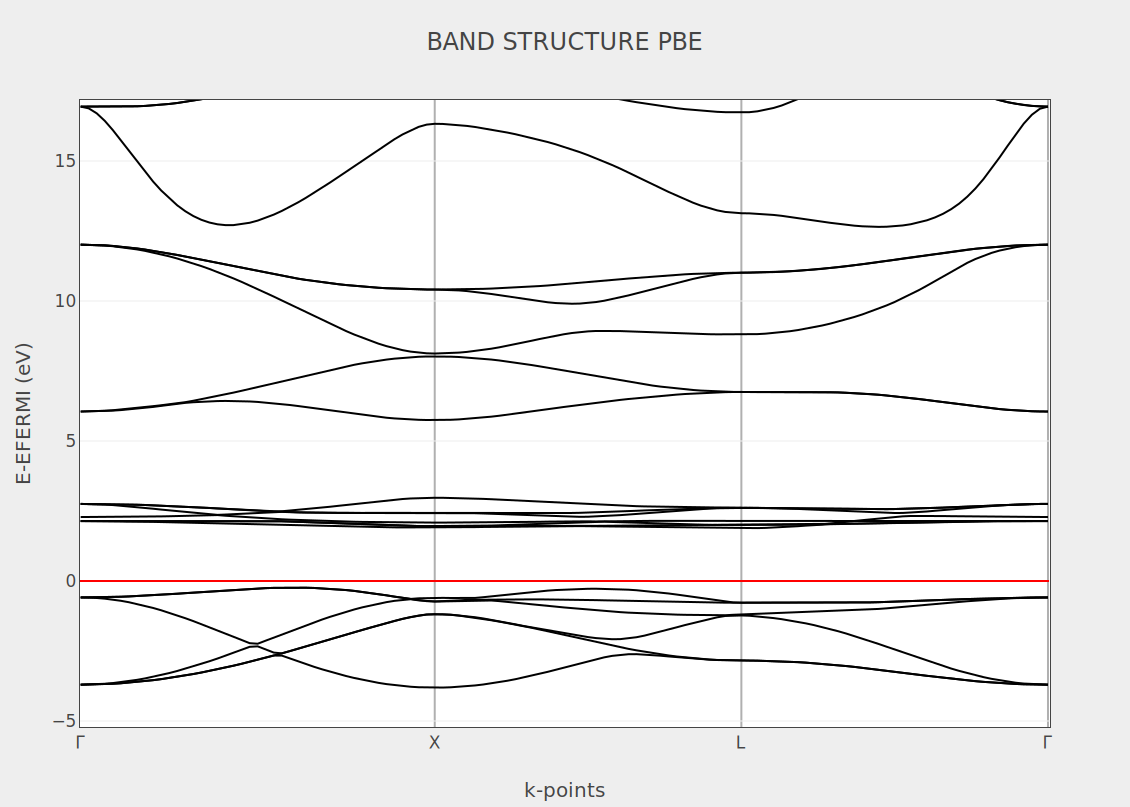
\includegraphics[width=1\textwidth]{../images/BANDS/BAND_STRUCTURE_PBE.jpeg}
	\captionof{figure}{Reported Band Structure of $CeO_2$ using PBE}
    \label{fig:bands_PBE}
\end{minipage}

\noindent\begin{minipage}{0.45\textwidth}
	\centering
	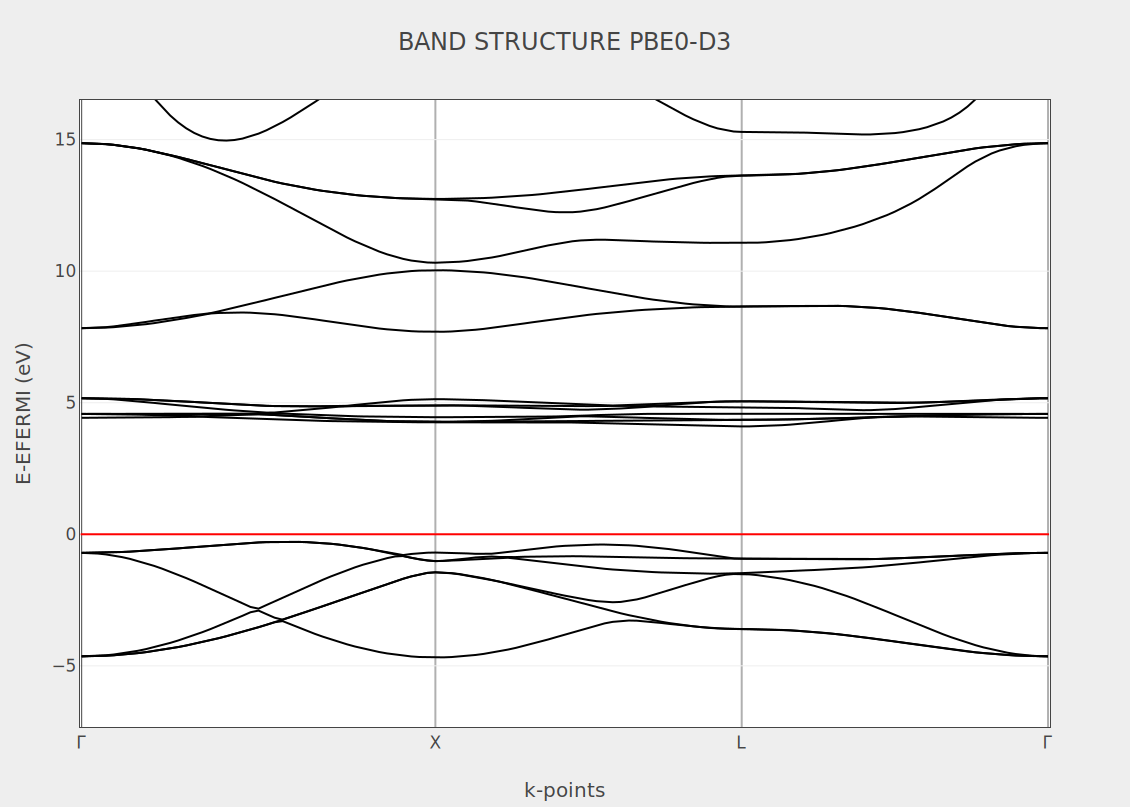
\includegraphics[width=1\textwidth]{../images/BANDS/BAND_STRUCTURE_PBE0D3.jpeg}
	\captionof{figure}{Reported Band Structure of $CeO_2$ using PBE0-D3}
    \label{fig:bands_PBE0D3}
\end{minipage}
\hfill
\begin{minipage}{0.45\textwidth}
	\centering
	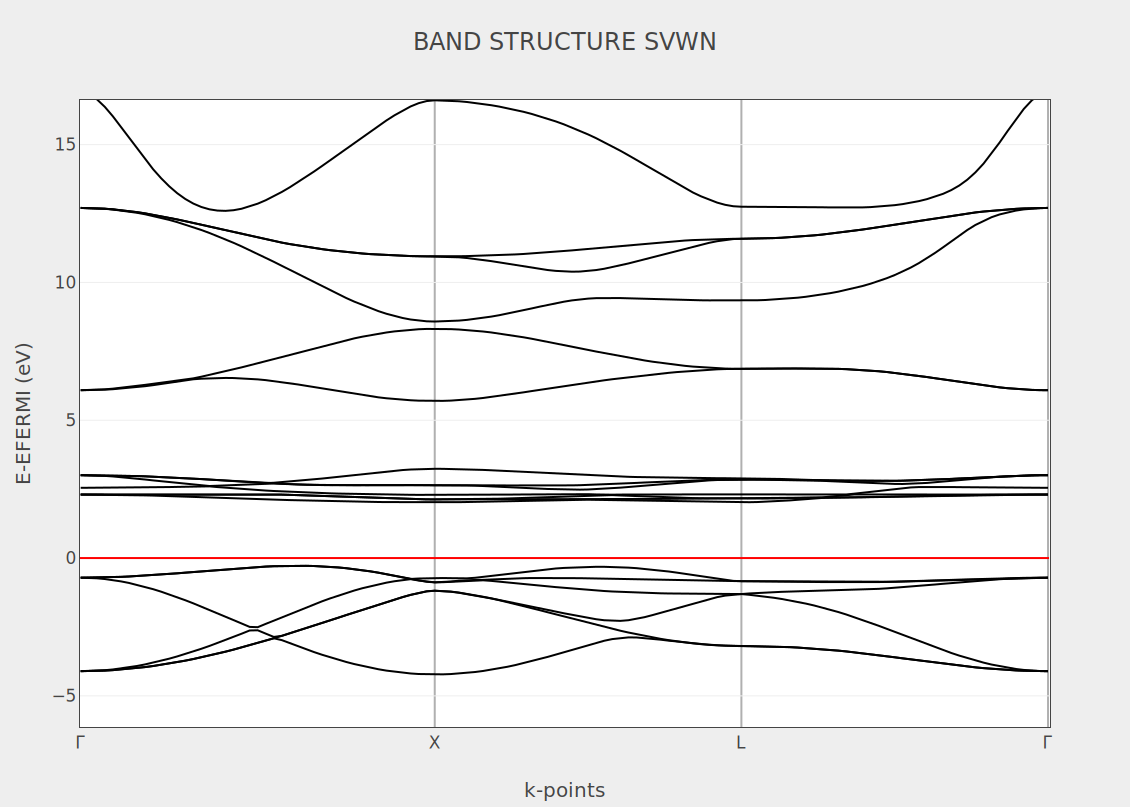
\includegraphics[width=1\textwidth]{../images/BANDS/BAND_STRUCTURE_SVWN.jpeg}
	\captionof{figure}{Reported Band Structure of $CeO_2$ using SVWN}
    \label{fig:bands_SVWN}
\end{minipage}

\newpage
\section{Density of States}

Once again, the same pattern emerges in different functionals regarding the spacing between the bands (Band Gap). What is highlighted is that despite the spacing, the form of the DOS is mantained across different functionals, meaning that the DOS structure overall is almost the same, just spread differentely.

From the plots it's possible to notice that the contribution to the valence band is mainly given by the \textit{p}-orbitals of the oxygen, while the conduction band is formed from the \textit{d} and \textit{f}-orbitals of Cerium.

\vspace{15pt}

\noindent\begin{minipage}{0.49\textwidth}
	\centering
	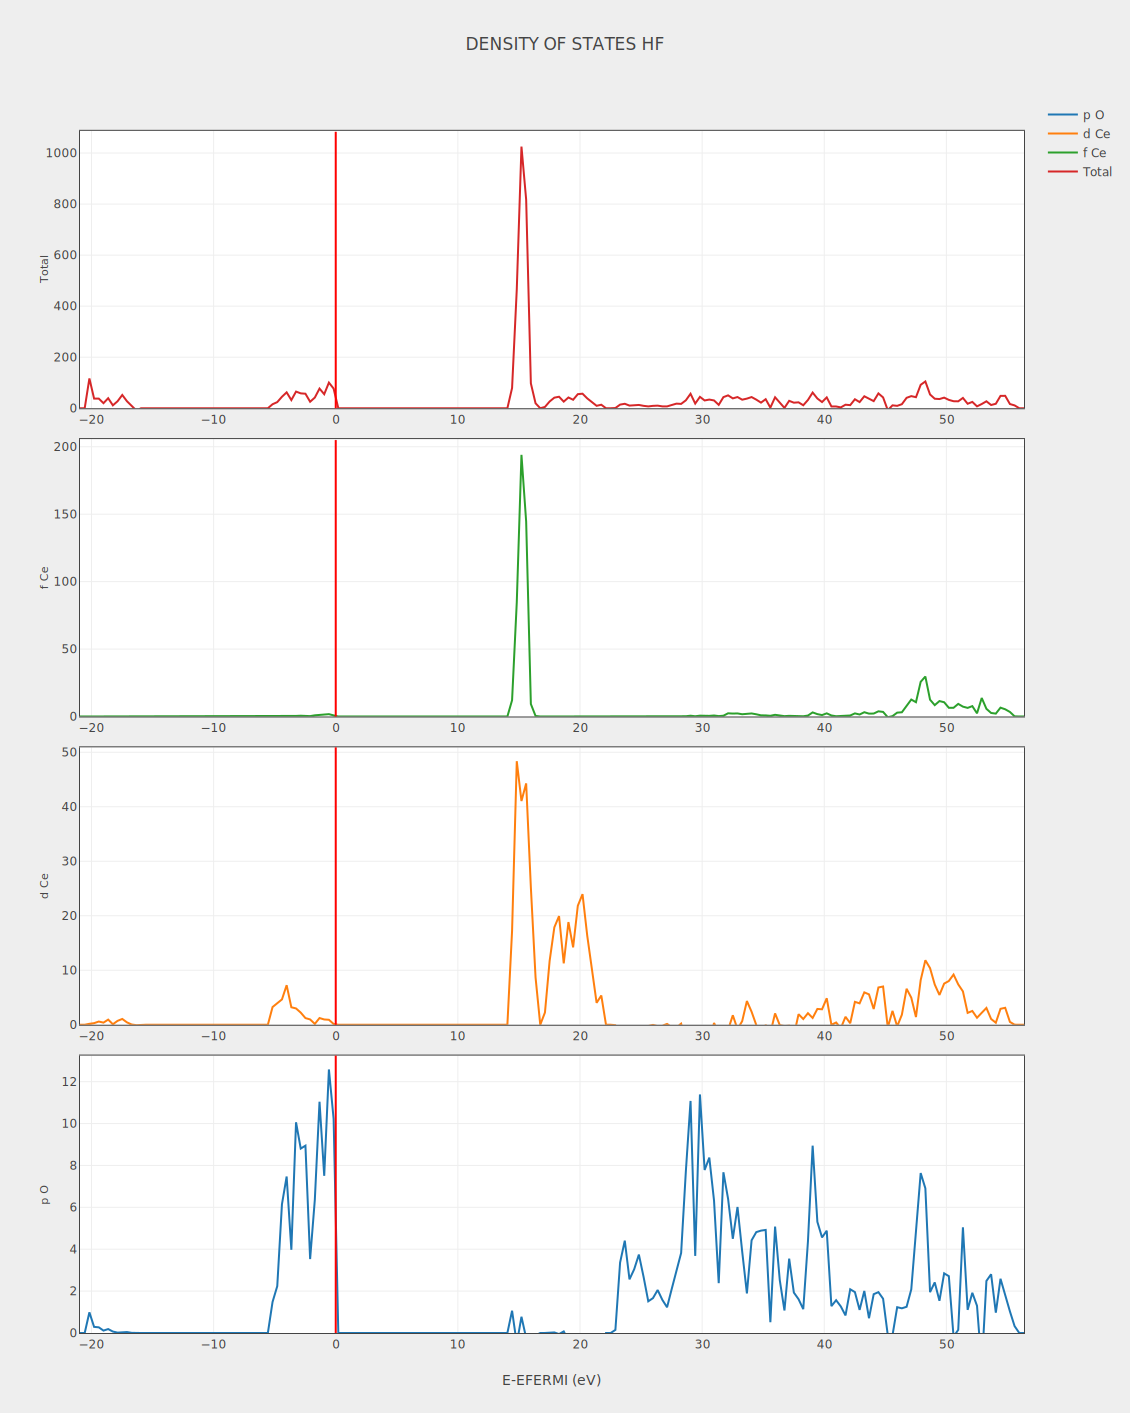
\includegraphics[width=1\textwidth]{../images/correct_band_and_dos/DOSS HF.jpeg}
	\captionof{figure}{DOS of $CeO_2$ using HF}
    \label{fig:DOS_HF}
\end{minipage}
\hfill
\begin{minipage}{0.49\textwidth}
	\centering
	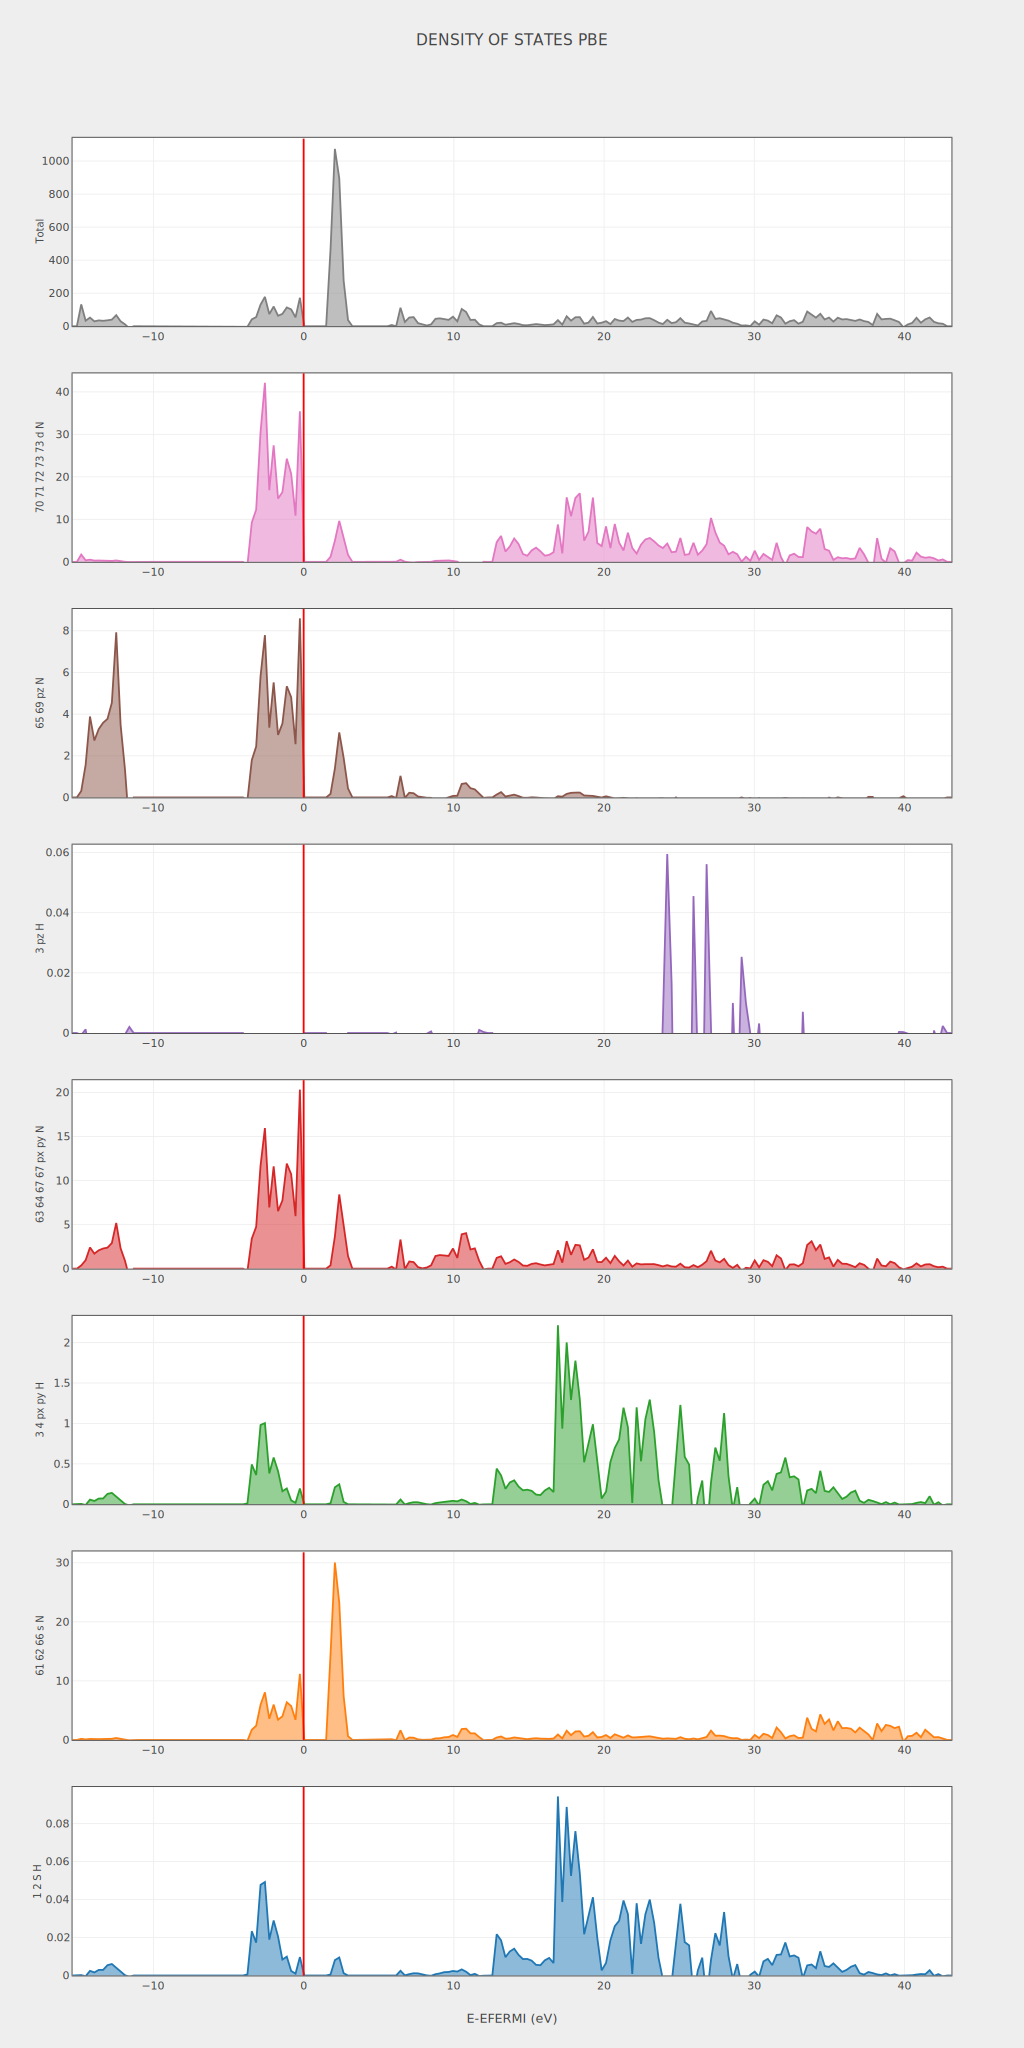
\includegraphics[width=1\textwidth]{../images/correct_band_and_dos/DOSS PBE.jpeg}
	\captionof{figure}{DOS of $CeO_2$ using PBE}
    \label{fig:DOS_PBE}
\end{minipage}

\noindent\begin{minipage}{0.49\textwidth}
	\centering
	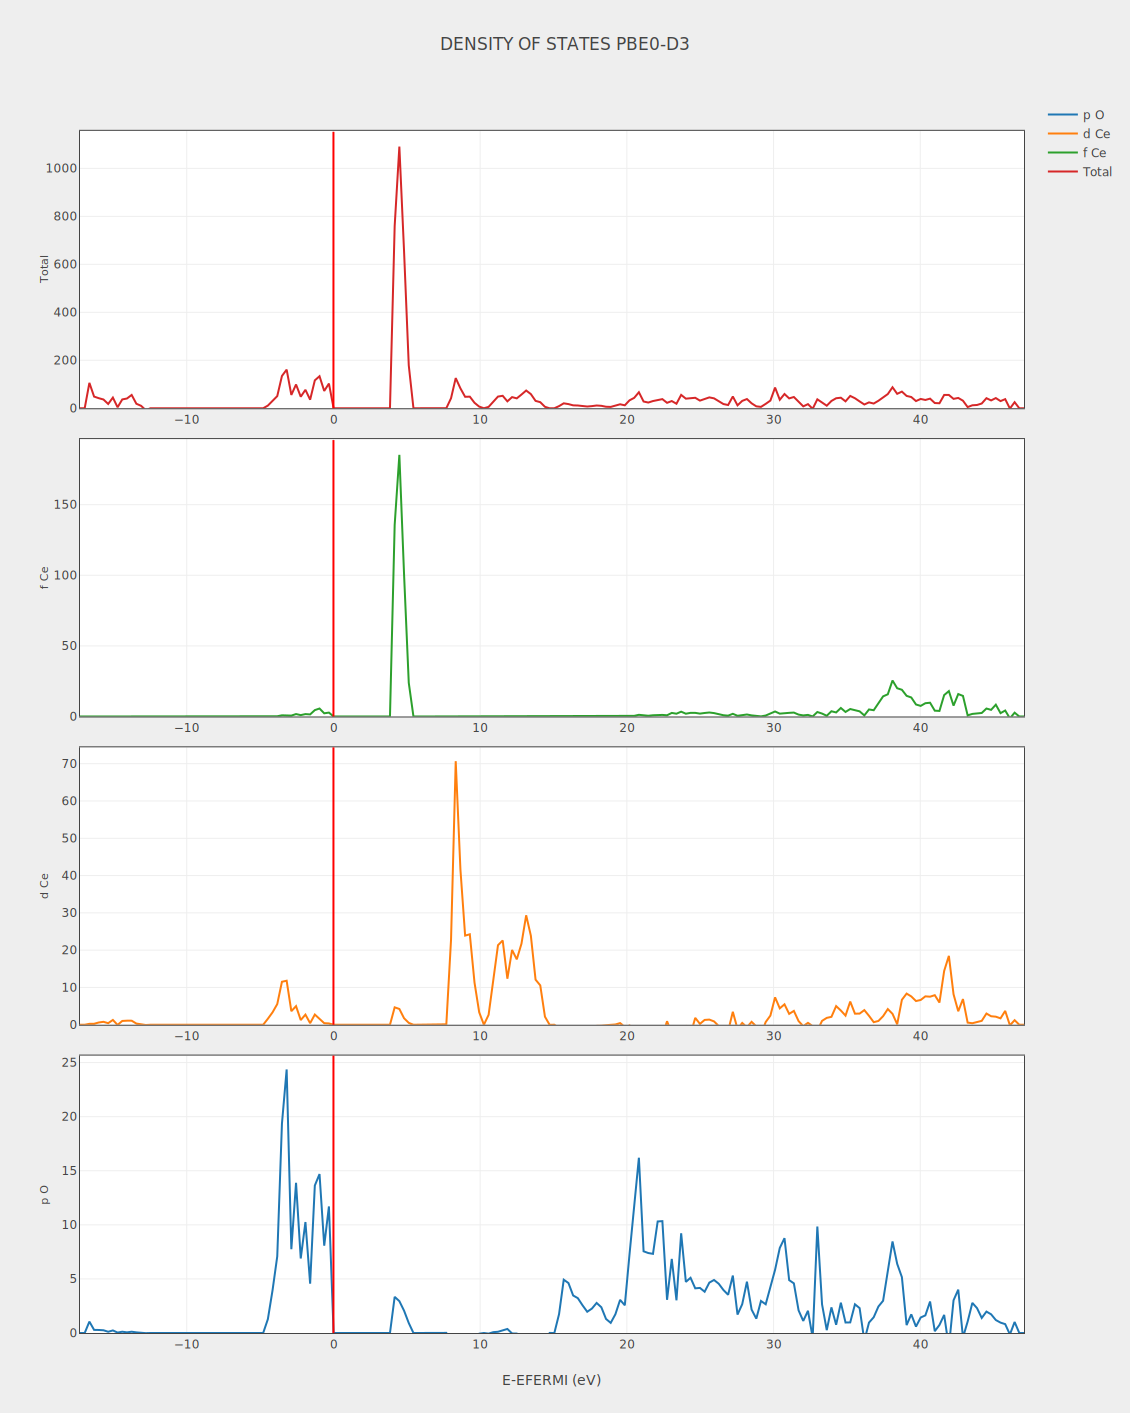
\includegraphics[width=1\textwidth]{../images/correct_band_and_dos/DOS PBE0-D3.jpeg}
	\captionof{figure}{DOS of $CeO_2$ using PBE0-D3}
    \label{fig:DOS_PBE0D3}
\end{minipage}
\hfill
\begin{minipage}{0.49\textwidth}
	\centering
	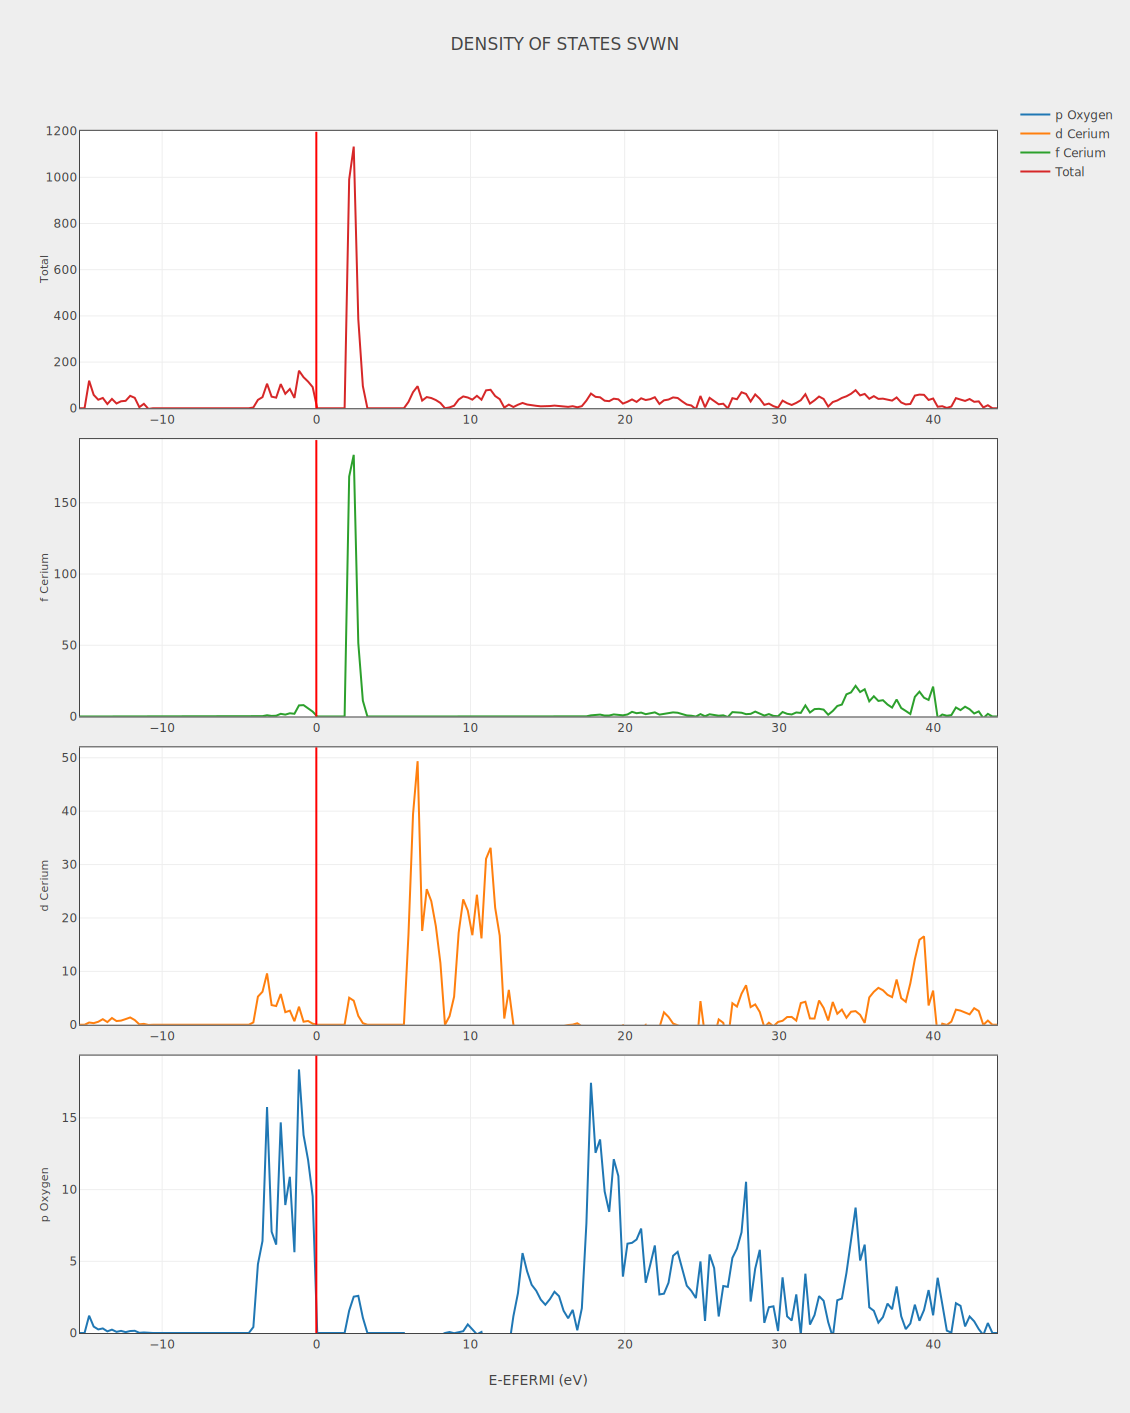
\includegraphics[width=1\textwidth]{../images/correct_band_and_dos/DOS SVWN.jpeg}
	\captionof{figure}{DOS of $CeO_2$ using SVWN}
    \label{fig:DOS_SVWN}
\end{minipage}

\newpage
\section{Unified Band Structure and Density of States}

For a more effective interpretation of the energy levels, here are reported the Band structure and Density of States next to each other.

\vspace{15pt}

\noindent\begin{minipage}{0.45\textwidth}
	\centering
	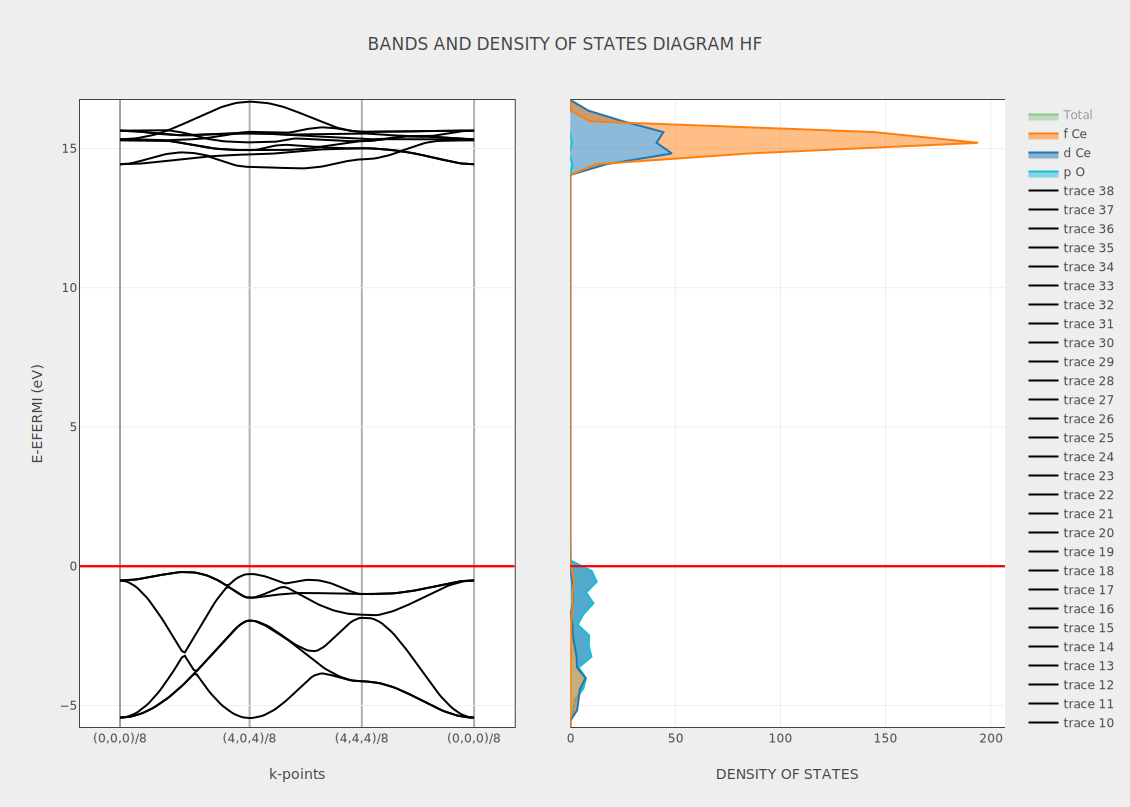
\includegraphics[width=1\textwidth]{../images/correct_band_and_dos/BAND AND DOSS HF.jpeg}
	\captionof{figure}{Reported Band Structure and Density of States of $CeO_2$ using HF}
    \label{fig:BANDDOS_HF}
\end{minipage}
\hfill
\begin{minipage}{0.45\textwidth}
	\centering
	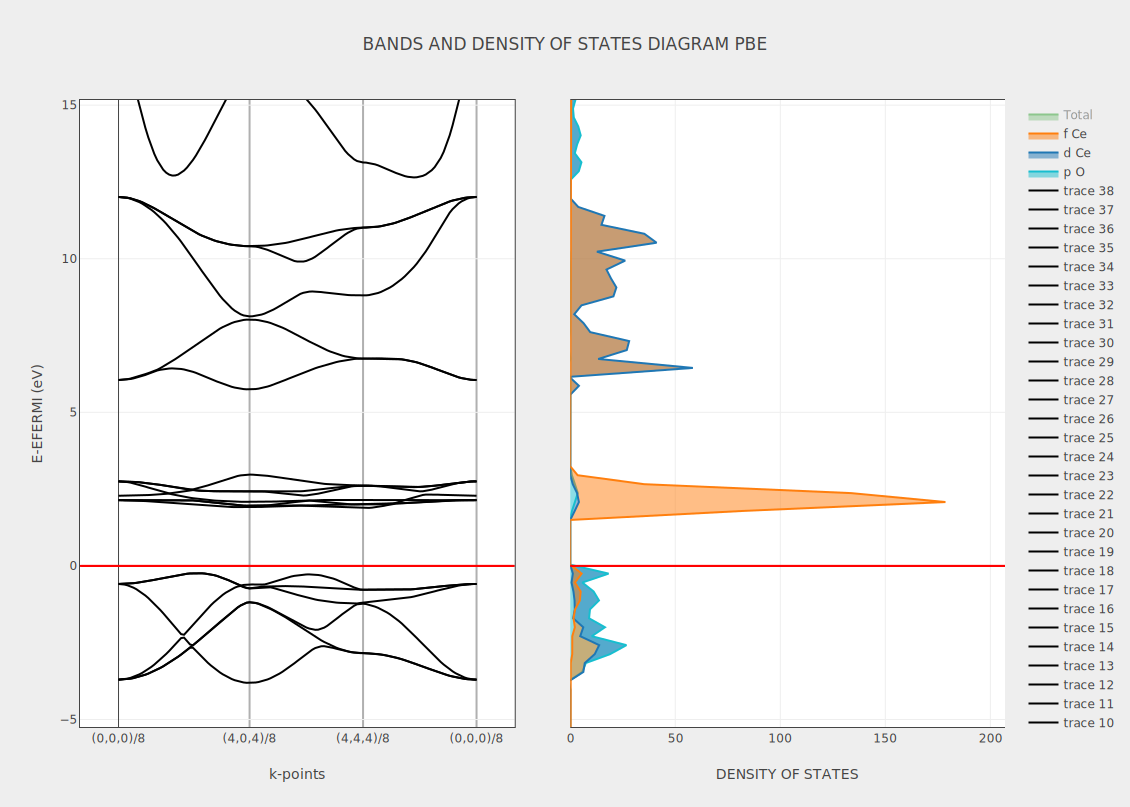
\includegraphics[width=1\textwidth]{../images/correct_band_and_dos/BAND AND DOSS PBE.jpeg}
	\captionof{figure}{Reported Band Structure and Density of States of $CeO_2$ using PBE}
    \label{fig:BANDDOS_PBE}
\end{minipage}

\noindent\begin{minipage}{0.45\textwidth}
	\centering
	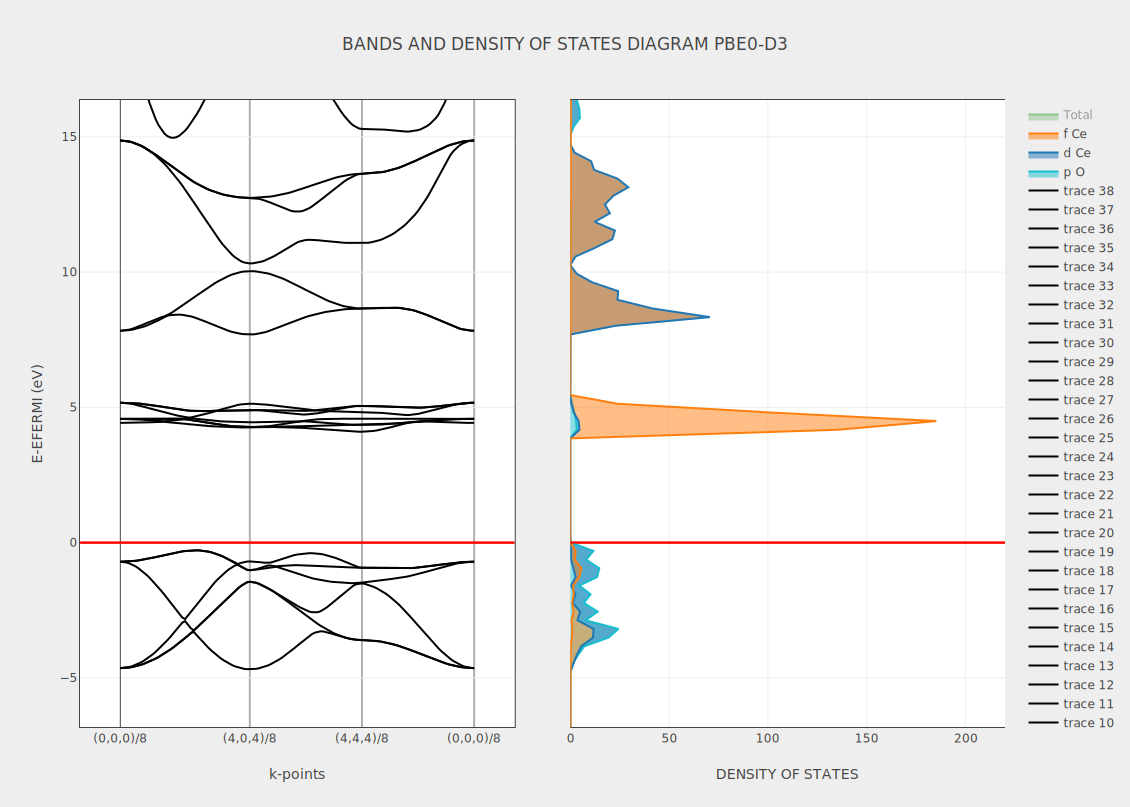
\includegraphics[width=1\textwidth]{../images/correct_band_and_dos/BAND AND DOSS PBE0-D3.jpeg}
	\captionof{figure}{Reported Band Structure and Density of States of $CeO_2$ using PBE0-D3}
    \label{fig:BANDDOS_PBE0D3}
\end{minipage}
\hfill
\begin{minipage}{0.45\textwidth}
	\centering
	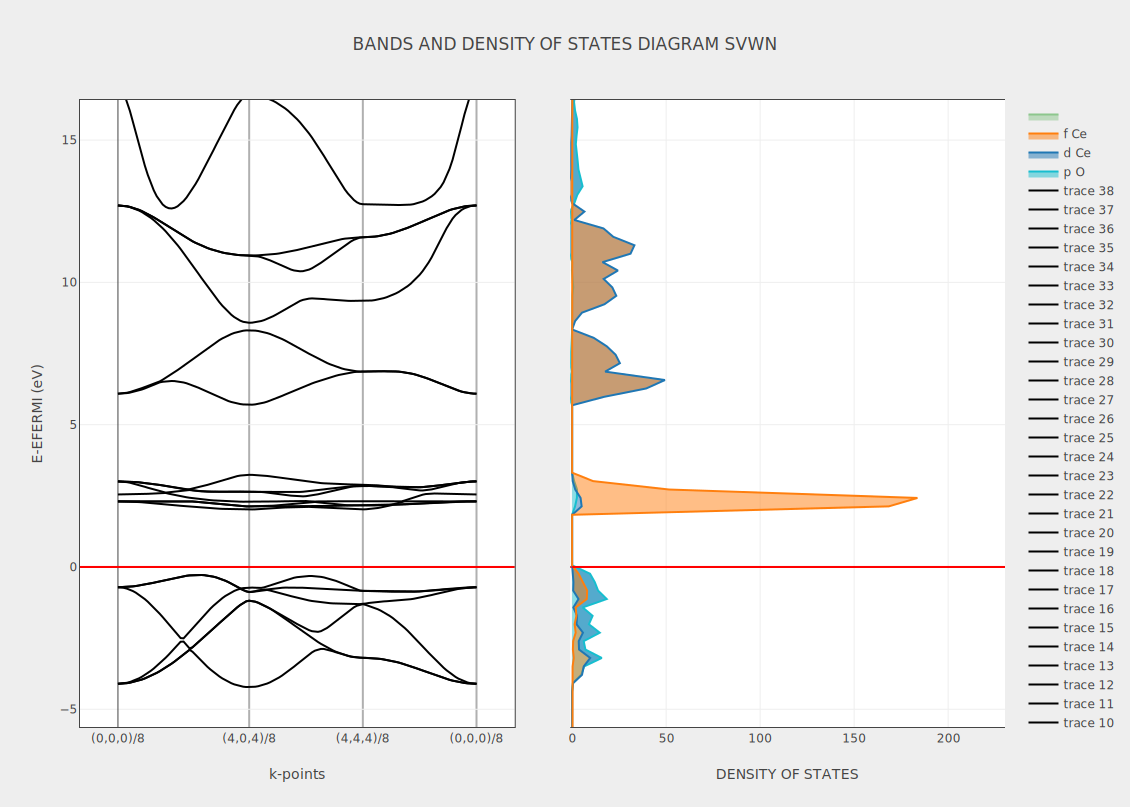
\includegraphics[width=1\textwidth]{../images/correct_band_and_dos/BAND AND DOSS SVWN.jpeg}
	\captionof{figure}{Reported Band Structure and Density of States of $CeO_2$ using SVWN}
    \label{fig:BANDDOS_SVWN}
\end{minipage}

\newpage
\section{Charge Density (Difference)}

By calculating che charge density difference, very similar results are obtained across different functionals. In Fig.\ref{fig:CHARGE_HF} observing the red ring in $Ce$, it is possible to notice a homogeneous charge distribution, leading to a smoother area. Conversely, in Fig.\ref{fig:CHARGE_PBE}, the same red ring is much more sharper. This difference may be attributed to the type of functional:
\begin{itemize}
	\item \textbf{Smoother}: HF $\rightarrow$ Delocalized atoms, leading to a bigger interaction and overlap.
	\item \textbf{Sharper}: PBE $\rightarrow$ Localized atoms and smaller overlap, might be the reason behind this stronger directionality. 
\end{itemize}
The other functionals appear to exhibit behavior that falls between HF and PBE, probably due to the mixed approach.

\vspace{15pt}

\noindent\begin{minipage}{0.45\textwidth}
	\centering
	\includegraphics[width=1\textwidth]{../images/DIFFERENCE CHARGE DENSITY/DIFF CHARGE DENSITY HF.jpeg}
	\captionof{figure}{Reported Charge Density Difference of $CeO_2$ using HF}
	\label{fig:CHARGE_HF}
\end{minipage}
\hfill
\begin{minipage}{0.45\textwidth}
	\centering
	\includegraphics[width=1\textwidth]{../images/DIFFERENCE CHARGE DENSITY/DIFF CHARGE DENSITY PBE.jpeg}
	\captionof{figure}{Reported Charge Density Difference of $CeO_2$ using PBE}
	\label{fig:CHARGE_PBE}
\end{minipage}

\noindent\begin{minipage}{0.45\textwidth}
	\centering
	\includegraphics[width=1\textwidth]{../images/DIFFERENCE CHARGE DENSITY/DIFF CHARGE DENSITY PBE0-D3.jpeg}
	\captionof{figure}{Reported Charge Density Difference of $CeO_2$ using PBE0-D3}
	\label{fig:CHARGE_PBE0D3}
\end{minipage}
\hfill
\begin{minipage}{0.45\textwidth}
	\centering
	\includegraphics[width=1\textwidth]{../images/DIFFERENCE CHARGE DENSITY/DIFF CHARGE DENSITY SVWN.jpeg}
	\captionof{figure}{Reported Charge Density Difference of $CeO_2$ using SVWN}
	\label{fig:CHARGE_SVWN}
\end{minipage}

\newpage
\section{Vibrational spectra}
From the calculated infrared vibrational spectra, it is evident that the characteristic frequency of the Ce-O bond is consistent across all four functionals, while the intensity increases in the following order: HF, PBE0-D3, SVWN, and PBE. Once again, HF and PBE represent the limiting cases, while the intermediate functionals exhibit properties that reflect a balance between these two. 

Unfortunately, there are no reference in literature reguarding this specific frequency, (no results below 400 cm$^{-1}$). From the animation in Crysplot, it seems to be a bending mode, but no further informations are present.

In the appendix the code used is reported, an error might have occured.

\vspace{15pt}

\noindent\begin{minipage}{0.45\textwidth}
	\centering
	\includegraphics[width=1\textwidth]{../images/IR/IR_HF.png}
	\captionof{figure}{Reported IR spectra of $CeO_2$ using HF}
	\label{fig:VIBRATIONAL_HF}
\end{minipage}
\hfill
\begin{minipage}{0.45\textwidth}
	\centering
	\includegraphics[width=1\textwidth]{../images/IR/IR_PBE.png}
	\captionof{figure}{Reported IR spectra of $CeO_2$ using PBE}
	\label{fig:VIBRATIONAL_PBE}
\end{minipage}

\noindent\begin{minipage}{0.45\textwidth}
	\centering
	\includegraphics[width=1\textwidth]{../images/IR/IR_PBE0_D3.png}
	\captionof{figure}{Reported IR spectra of $CeO_2$ using PBE0-D3}
	\label{fig:VIBRATIONAL_PBE0D3}
\end{minipage}
\hfill
\begin{minipage}{0.45\textwidth}
	\centering
	\includegraphics[width=1\textwidth]{../images/IR/IR_SVWN.png}
	\captionof{figure}{Reported IR spectra of $CeO_2$ using SVWN}
	\label{fig:VIBRATIONAL_SVWN}
\end{minipage}



\newpage
\section{Conclusions}
In this work 4 different functionals were used, here's a brief overview:
\begin{itemize}
	\item \textbf{HF}: A good starting point, but typically very computationally expensive. It often provides significantly incorrect band-gap predictions due to the lack of electron correlation.
	\item \textbf{PBE}: A fast and efficient method, but tends to underestimate the band-gap.
	\item \textbf{PBE0-D3}: A hybrid functional combining 25\% Hartree-Fock exchange with PBE, yielding more accurate overlap and improving results for weak interactions due to the inclusion of the D3 dispersion correction. However, it often incurs into a significant computational cost.
	\item \textbf{SVWN}: Generally a little less accurate than the PBE0-D3 for the current system. It remains the second-fastest functional and provides a better description of exchange-correlation interactions compared to PBE and HF.
\end{itemize}

\noindent The best functional (given the results), would be the \textbf{PBE0-D3}, a very good solution for different properties. However, to obtain a fast execution time and generally a good accuracy, \textbf{SVWN} has the best trade-off between speed and accuracy.

\newpage
\section{Appendix}

In the following pages are reported all the input files used. They all refer to the \textbf{SVWN} functional.

\vspace{20pt}

\noindent\begin{minipage}[t]{0.45\textwidth}
    \textbf{main\_input.d12}
    \vspace{15pt}
	\\CeO2
	\\CRYSTAL
	\\0 0 0 
	\\225
	\\5.47
	\\2
	\\258 0 0 0
	\\8 0.25 0.75 0.75
	\\OPTGEOM
	\\END
	\\END
	\\\%\% BASIS SET START \%\%
	\\Ce\_pob\_TZVP\_rev2
	\\O\_pob\_TZVP\_rev2
	\\\%\% BASIS SET END \%\%
	\\99 0
	\\END
	\\DFT
	\\SVWN
	\\END
	\\SHRINK
	\\8 8
	\\MULPOPAN
	\\END
\end{minipage}
\hfill
\begin{minipage}[t]{0.45\textwidth}
    \textbf{CHARGE\_DIFFERENCE.d3}
    \vspace{15pt}
	\\ECHG
	\\0
	\\100
	\\COORDINA
	\\-4. -4. 0.0
	\\4. -4. 0.0
	\\4. 4. 0.0
	\\MARGINS
	\\2.0 2.0 2.0 2.0
	\\END
	\\PATO
	\\0 0
	\\ECHG
	\\0
	\\100
	\\COORDINA
	\\-4. -4. 0.0
	\\4. -4. 0.0
	\\4. 4. 0.0
	\\MARGINS
	\\2.0 2.0 2.0 2.0
	\\END
	\\END
\end{minipage}

\vspace{20pt}

\noindent\begin{minipage}[t]{0.45\textwidth}
    \textbf{BAND.d3}
    \vspace{15pt}
	\\BAND
	\\Path G X L G
	\\3 8 120 15 53 1 0
	\\0 0 0   4 0 4
	\\4 0 4   4 4 4
	\\4 4 4   0 0 0
	\\END
    
\end{minipage}
\hfill
\begin{minipage}[t]{0.45\textwidth}
	\textbf{DOS.d3}
	\vspace{15pt}
	\\NEWK
	\\8 8
	\\1 0
	\\DOSS
	\\3 200 15 53 1 14 0
	\\3   72 73 74
	\\5   36 37 38 39 40
	\\7   55 56 57 58 59 60 61
	\\END
\end{minipage}

\begin{minipage}[t]{0.45\textwidth}
	\textbf{vibrational\_input.d12}
	
	\vspace{15pt}
	
	CeO2
	\\CRYSTAL
	\\0 0 0 
	\\225
	\\5.47
	\\2
	\\258 0 0 0
	\\8 0.25 0.75 0.75
	\\FREQCALC
	\\INTENS
	\\END
	\\END
	\\\%\% BASIS SET START \%\%
	\\Ce\_pob\_TZVP\_rev2
	\\O\_pob\_TZVP\_rev2
	\\\%\% BASIS SET END \%\%
	\\99 0
	\\END
	\\DFT
	\\SVWN
	\\END
	\\SHRINK
	\\8 8
	\\MULPOPAN
	\\END
	
\end{minipage}
\hfill
\begin{minipage}[t]{0.45\textwidth}
	\textbf{vibrational\_input\_restart.d12}
	
	\vspace{15pt}
	
	CeO2
	\\CRYSTAL
	\\0 0 0 
	\\225
	\\5.47
	\\2
	\\258 0 0 0
	\\8 0.25 0.75 0.75
	\\FREQCALC
	\\RESTART
	\\INTENS
	\\IRSPEC
	\\END
	\\END
	\\END
	\\\%\% BASIS SET START \%\%
	\\Ce\_pob\_TZVP\_rev2
	\\O\_pob\_TZVP\_rev2
	\\\%\% BASIS SET END \%\%
	\\99 0
	\\END
	\\DFT
	\\SVWN
	\\END
	\\SHRINK
	\\8 8
	\\MULPOPAN
	\\END


\end{minipage}

\newpage
\bibliographystyle{unsrt}
\bibliography{biblio}  

\end{document}